\documentclass[border=2mm]{standalone}
\usepackage{tikz}
\usepackage{mathtools}
% \usepackage{tikz-3dplot}
\usetikzlibrary{calc}

\begin{document}
% \tdplotsetmaincoords{70}{120}

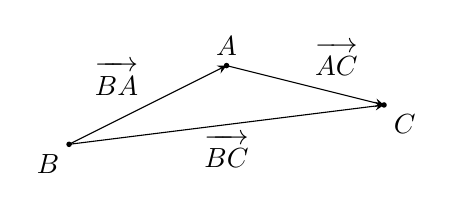
\begin{tikzpicture}[>=stealth]
  \coordinate (B) at (0,0);
  \coordinate (A) at (2,1);
  \coordinate (C) at (4,0.5);

  \draw[->] (B) -- (A) node[midway, above left] {$\overrightarrow{\vphantom{A^{A}}BA}$};

  \draw[->] (A) -- (C) node[midway, above right] {$\overrightarrow{\vphantom{A^{A}}AC}$};

  \draw[->] (B) -- (C) node[midway, below] {$\overrightarrow{\vphantom{A^{A}}BC}$};

  \fill (B) circle (1pt) node[below left] {$B$};

  \fill (A) circle (1pt) node[above] {$A$};

  \fill (C) circle (1pt) node[below right] {$C$};
\end{tikzpicture}

\end{document}